\subsection{Parameter optimization}\label{s_paropt}
\noindent In section \ref{s_optimalcontrol} it was made clear that with the chosen method increasing the dimensionality of the problem is feasible. The skateboards' parameters can be optimized as decision variables which increases the state space, but with direct methods this should not be a problem. It is similar to setting an initial value of a state free for optimization but now it will be a parameter defining the skateboards geometry. To optimize the geometry of the skateboard I made a parameterized model of the skateboard that scales it's mass and inertia values when changing the geometry, such that the dynamical response is scaled as well. I used the SymPy symbolic toolbox to create the parameterized models \cite{meurer_sympy_2017}. 

\subsubsection{Parameterized model}\label{ss_model}
%%%%%%%%%%%%%%%% begin figure %%%%%%%%%%%%%%%%%%%
\begin{figure}
\centerline{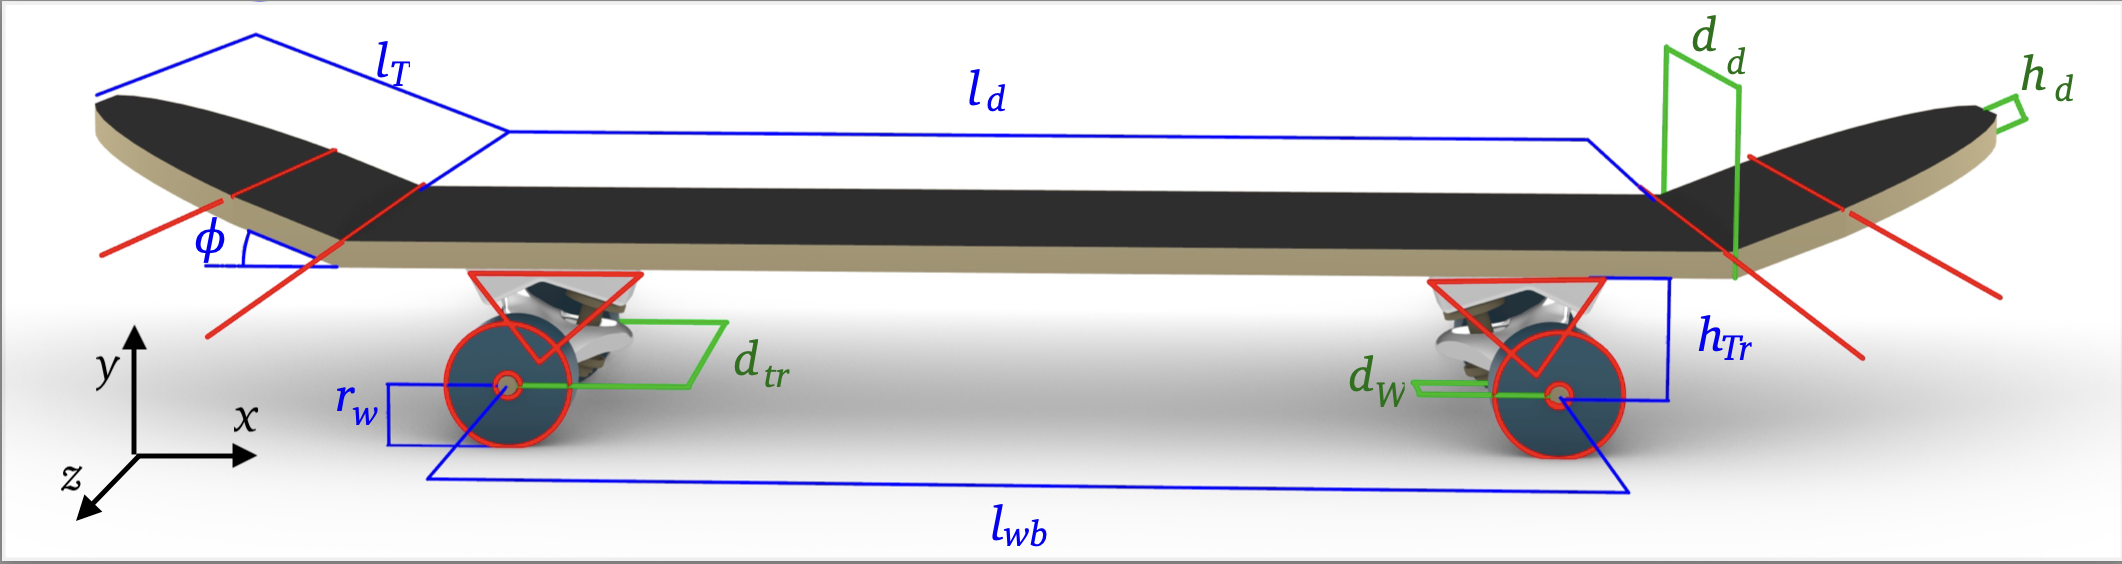
\includegraphics[width=0.5\textwidth,trim={0.1cm 0.1cm 0.1cm 0.05cm},clip]{figure/parameterized.png}}
\caption[11-Segment skateboard model]{Parameterized skateboard. Blue variables are located in the xy-plane. All blue variables except for $h_d$ and $d_{com}$ are optimized during the ollie optimization. Green variables are chosen by preference. Red lines split the skateboard into 11 basic shaped segments for inertia calculation (see figure \ref{f_basicshapes})}
\label{f_11segments}
\end{figure}
%%%%%%%%%%%%%%%% end figure %%%%%%%%%%%%%%%%%%%

\noindent The most widely accepted skateboard is the Popsicle stick skateboard (see section \ref{s_intro}). A simplification of the Popsicle stick skateboard is minimally described in ten variables. A symmetrical shape is assumed, whereas in reality nose and tail length and inclination often vary. The simplified skateboard is made up of straight lines only and concavity is not taken into account. An infinitely stiff skateboard is assumed as stated in section \ref{ss_mechanics}. Eight variables are located in the xy-plane shown in blue in fig.\ref{f_11segments}. Wheelbase ($l_{wb}$), deck length ($l_{d}$), length tail and nose ($l_{t}$), tail and nose inclination relative to the deck ($\phi$), truck height ($h_{tr}$), wheel radius ($r_{w}$), and COM distance from deck $d_{com}$. These will be the optimization variables because they affect the 2D kinematics of the ollie directly, except for $d_{com}$. As $d_{com}$ is a function of the other parameters. All other parameters are set at the industry standard or a measured value (see table \ref{t_typical}). Deck thickness ($h_d$) is dependent on the amount of layers of veneer that is used during production. All zx-plane related variables are shown in green in fig.\ref{f_11segments}. Truck width ($d_{tr}$), and wheel width ($d_w$), deck width ($d_d$). They are usually chosen by the skater through preference and won't be part of the optimization. Truck and deck width are assumed to be equal. This leads to the variables that will be optimized for improving the geometry of the skateboard during an ollie:
\begin{equation}
    [l_{wb},\ l_d,\ l_t,\ \phi,\ h_{tr},\ r_w ]
\end{equation}

\subsubsection{Mass distribution}\label{ss_mass}
\noindent The mass and it's distribution influence the dynamic response of the skateboard \cite{moore_force_nodate}. A mass model is made to be able to scale the mass and it's distribution when the optimized parameters are changed. The skateboards' COM is calculated as a composite of 11 basic constant density shapes shown in figure \ref{f_basicshapes}. The shapes consist of semi-cylinders, cuboids, cylinders and triangular prisms. To calculate the mass of each part, the volume of each segment is calculated and multiplied by it's density except for the trucks. For the trucks, density is calculated from a measured truck weight divided by the volume of the truck estimated as an triangular prism. The typical weight influencing properties are seen in table \ref{t_typical}. See appendix A for mass, inertia, and geometry calculations. 
\begin{figure}
    \centering
    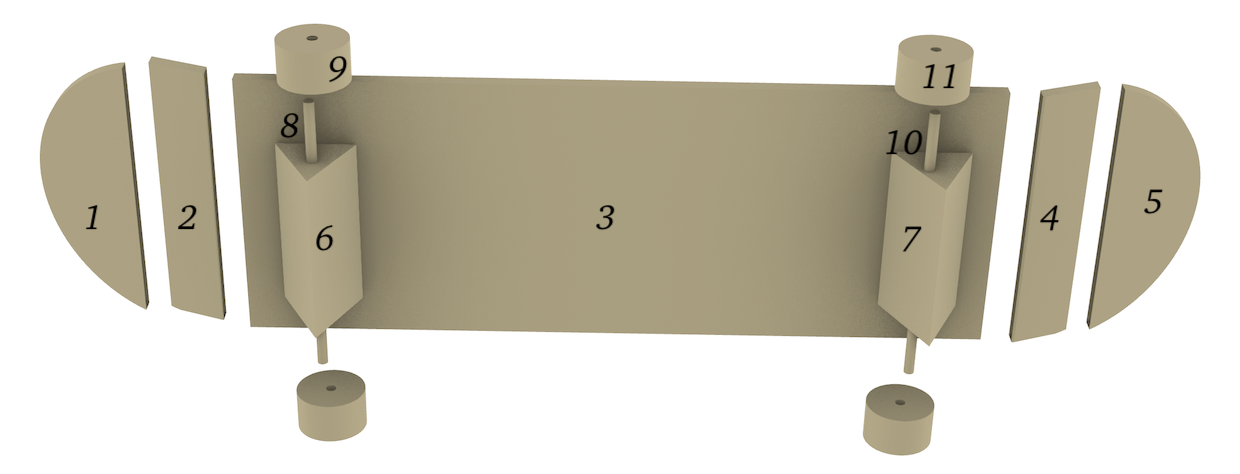
\includegraphics[width = 0.5 \textwidth]{figure/Basicshapes.png}
    \caption[Exploded 11 segment model]{Clarification on the 11 segment model. Now you can see that there are 13 shapes, but the wheels are taken as one wider cylinder in 2D, which results in 11 segments}
    \label{f_basicshapes}
\end{figure}
%%%%%%%%%%%%%%% begin table   %%%%%%%%%%%%%%%%
\begin{table}[t]
\begin{center}
\caption[Industry standard and measured skateboard dimensions]{Industry standards and measured values from a PolarSkate Co. deck with Independent trucks}
\label{t_typical}
\begin{tabular}{l l l}
& & \\ % put some space after the caption
\hline
Description & Variable & Value \\
\hline
Wheel density (PU) & $\rho_{pu}$    & $1130 \quad [\frac{kg}{m^3}]$ \footnotemark\\
Hard maple density & $\rho_{maple}$ & $705 \quad [\frac{kg}{m^3}]$ \footnotemark\\
Thickness veneer & $d_{veneer}$ & $0.0016 \quad [m]$ \footnotemark\\
Specific mass PVA glue & $s_{glues}$ & $0.105 \quad [\frac{kg}{m^2}]$ $^{3}$  \footnotemark  \\
Density steel & $\rho_{steel} $ & $ 7700 \quad [\frac{kg}{m^3}] $ \\
Radius axle & $r_{axle} $   & $0.004 \quad [m] ^*$ \\
Width deck & $d_{D}$ & $0.21 \quad [m] ^*$ \\
Number of ply's & $n_{ply}$  & $7 $ \\
Mass bearing & $m_{bearing} $ & $0.012 \quad [kg] ^*$ \\ 
Mass truck   & $m_{truck} $   & $0.366 \quad [kg] ^*$ \\
\hline
\multicolumn{3}{l}{$^{1}$ \scriptsize{\url{https://www.lorkindustrias.com/}}} \\ \noalign{\vskip -4mm}    
\multicolumn{3}{l}{$^{2}$ \scriptsize{\url{https://www.wood-database.com/hard-maple/}}} \\ \noalign{\vskip -4mm}
\multicolumn{3}{l}{$^{3}$ \scriptsize{\url{https://www.timberaid.com/}}} \\ \noalign{\vskip -4mm}
\multicolumn{3}{l}{$^{4}$ \scriptsize{\url{http://www.franklinadhesivesandpolymers.com}}} \\ \noalign{\vskip -4mm}
\multicolumn{3}{l}{$^{*}$ \scriptsize{Measured with caliper (+-0.1mm) or with scale (+-1gram)}} \\ \noalign{\vskip -4mm}
\end{tabular}
\end{center}
\end{table}
%%%%%%%%%%%%%%%% end table %%%%%%%%%%%%%%%%%%%

%%%%%%%%%%%%%%% begin table   %%%%%%%%%%%%%%%%
\begin{table}
\begin{center}
\caption[Inertia]{Formulas of volume and inertia of each basic shape to calculate skateboards inertia. $l=$ length, $d=$ width, $r=$ radius L = length of isosceles, $\beta$ = top angle of isosceles}
\label{t_volume_inert}
\begin{tabular}{c l p{1.06in}}
& & \\ % put some space after the caption
\hline
Shape & Volume & Inertia \\
\hline
Cuboid           & $l\cdot d\cdot h$              & $\frac{m}{12} (l_x^2+l_y^2)$ \\
Triangular prism & $\frac{1}{2} l\cdot d\cdot h$  &  $\frac{1}{2} m L^2\left(1-\frac{2}{3} \sin ^2 \beta\right)$ \cite{morin_introduction_2008}\\
Cylinder         & $\pi h (R^2-r^2)$                        &  $I_{x},I_{y} = \frac{m}{12} (3 r^2 + l^2)$ $I_{z} = \frac{r^2}{2 m} $ \\
Semi-cylinder    & $\frac{1}{2}\pi h (R^2-r^2)$             &  $(\frac{1}{4}-\frac{16}{9 \pi^2}) m r^2)$ \\
\hline

\end{tabular}

\end{center}
\end{table}
%%%%%%%%%%%%%%%% end table %%%%%%%%%%%%%%%%%%%


\subsubsection{Inertia}\label{ss_inertia}
\noindent To know the dynamic rotational response of the skateboard, the inertia about the skateboards' COM is needed. When the optimized parameters change the inertia should scale accordingly. A simplified inertia is calculated from the basic shapes found in figure \ref{f_11segments}. Inertia's about the COM of each segment can be found in table \ref{t_volume_inert}. The total inertia about the COM of the skateboard is calculated with the parallel axis theorem:

\begin{equation}
    I_{total} = \sum_{i=1}^{11} I_i + m_i  |\vec r_{i/com}| ^2
\end{equation}

\noindent A series of measurements is performed to validate the inertia model. For more detailed information on the inertia model and inertia measurement see Appendix A
% \paragraph{Verification}
% To make sure the theoretical models are valid, the mass en inertia of two arbitrary skateboards are measured. 
% \paragraph{Inertia measurement}
% The moment of inertia of the two skateboards are measured by hanging the parts as a compound pendulum and measuring their periods of oscillation. A similar method has been shown effective by Moore \cite{moore_accurate_2010}.

% For the simulation only the inertia about the COM in the xy-plane is necessary. 

% When considering a compound pendulum in a 2D-plane with friction, the torque acting on the system due to the gravity is:

% \begin{equation} \label{torque}
%     \tau = -L m g sin(\theta) + c L \dot sin(\theta)
% \end{equation}
% Eulers second law of motion with a fixed origin reduces to $\sum M_o = I_o \Ddot \theta $. Assuming small angles \ref{torque} can be written as:
% \begin{equation}
%     \Ddot \theta I_o = -L m g \theta + c L \dot sin(\theta)
% \end{equation}

% Pendulum
% How measurement is done

